% === C04 - Interrupciones externas ===
% David Alejandro Gonzalez Marquez
% dmarquez@dc.uba.ar / fokerman@gmail.com
% https://github.com/fokerman/Orga2Course

\documentclass[aspectratio=169]{beamer}
% \documentclass[handout]{beamer}

% % % Packages
\usepackage[sfdefault]{AlegreyaSans}
\usepackage{inconsolata}
\usepackage{multicol}
\usepackage{multirow}
\usepackage[spanish]{babel}
\usepackage[utf8]{inputenc}
\usepackage{enumerate}
\usepackage{color}
\usepackage{xcolor}
\usepackage[absolute,overlay]{textpos}
  \setlength{\TPHorizModule}{1mm}
  \setlength{\TPVertModule}{1mm}
\usepackage{framed}
\usepackage{mfirstuc} % para poner en mayusculas la primer letra
\usepackage{xspace} % para crear espacios en comandos 
\usepackage{pbox}
\usepackage{tikz}
\usepackage{mathabx}

% % % Beamer config
\usetheme{Pittsburgh}
\usecolortheme[rgb={1,0.48,0.0}]{structure}
\setbeamercolor{block title}{fg=white,bg=verdeuca}
\xdefinecolor{verdeuca}{rgb}{0.0,0.48,0.54}
\xdefinecolor{naranjauca}{rgb}{1,0.48,0.0}
\setbeamercolor{palette quaternary}{fg=white,bg=verdeuca}
\setbeamertemplate{title page}[default][colsep=-4bp, rounded=true] % remove title shadow
\setbeamertemplate{frametitle}[default][colsep=-2bp, shadow=false] % remove frame title shadow
\setbeamertemplate{navigation symbols}{} % remove navigation symbols
\beamertemplatenavigationsymbolsempty

% % % Colors
\definecolor{AzulClaro}{rgb}{.31,.506,.741}
\definecolor{Gris}{gray}{0.8}
\definecolor{Celeste}{rgb}{.255,.41,.884}
\definecolor{Rojo}{rgb}{1, 0, 0}
\definecolor{a}{rgb}{0.0, 0.53, 0.74}
\definecolor{r}{rgb}{0.89, 0.0, 0.13}
\definecolor{v}{rgb}{0.0, 0.5, 0.0}
\definecolor{y}{rgb}{0.0, 0.5, 0.5}
\definecolor{rojo}{HTML}{F1521B}
\definecolor{verde}{HTML}{80CD29}
\definecolor{amarillo}{HTML}{FABC09}
\definecolor{azul}{HTML}{00ADF1}

% % % Rename
\newcommand{\tab}[0]{\hspace{15pt}}

% % % Blocks
\setbeamercolor{block body}{fg=black, bg=black!10}
\setbeamercolor{block title}{fg=black, bg=black!20}
\setbeamercolor{coloredboxstuffNaranja}{fg=naranjauca,bg=black!10} %% PARA LOS BOX
\setbeamercolor{coloredboxstuffVerde}{fg=verdeuca,bg=black!10} %% PARA LOS BOX

% % % Start

\title{\Huge Interrupciones Externas}
\subtitle{Programación de Sistemas Operativos}
      
\author{David Alejandro González Márquez}
\institute{Departamento de Computación\\
Facultad de Ciencias Exactas y Naturales\\
Universidad de Buenos Aires}
\date{}

\begin{document}

\frame[plain]{\titlepage}

\begin{frame}
    \frametitle{Controlador de Interrupciones}
    \large
    \begin{itemize}
    \setlength\itemsep{0.8cm}
    \item[-] Una PC compatible posee mínimamente los siguientes dispositivos:
        \begin{itemize}    \large
            \item[$\cdot$] \textcolor{verdeuca}{\texttt{8259} - Controlador de Interrupciones}
            \item[$\cdot$] \textcolor{verdeuca}{\texttt{8254} - Timer Tick}
            \item[$\cdot$] \textcolor{verdeuca}{\texttt{8042} - Controlador del Teclado}
        \end{itemize}
    \pause
    \item[-] Tanto \textbf{Timer Tick} como el \textbf{Controlador del Teclado}, están conectados al Controlador de Interrupciones a \texttt{IRQ0} y \texttt{IRQ1} respectivamente.
    \pause
    \item[-] En realidad, se poseen dos controladores de interrupciones conectados en cascada, mapeados a las interrupciones a partir del índice \texttt{08h}
    \end{itemize}
\end{frame}

\begin{frame}
    \frametitle{Configuración de PIC 8259}
    \begin{itemize} \large
    \setlength\itemsep{0.6cm}
    \item[-] Las interrupciones por hardware del procesador, \textbf{se pisan} con los indices\\ seteados para los controladores de interrupciones.
    \pause
    \item[-] Se deben \textbf{remapear} los controladores a un espacio de interrupciones\\ designado a dispositivos de entrada/salida.
    \pause
    \item[-] Para acceder a los \texttt{PIC} se usan las instrucciones ``\texttt{in}'' y ``\texttt{out}''.
    \pause
    \item[-] La direcciones \texttt{20h} y \texttt{21h} corresponden al \texttt{PIC1}, y las direcciones \texttt{A0h} y \texttt{A1h} al \texttt{PIC2}
    \end{itemize}
\end{frame}

\begin{frame}
    \frametitle{Configuración de PIC 8259}
    \begin{textblock}{100}(10,15) \only<1->{\includegraphics[scale=0.52]{img/pic-layer1.pdf}} \end{textblock}
    \begin{textblock}{100}(10,15) \only<2->{\includegraphics[scale=0.52]{img/pic-layer2.pdf}} \end{textblock}
    \begin{textblock}{100}(10,15) \only<3->{\includegraphics[scale=0.52]{img/pic-layer3.pdf}} \end{textblock}
    \begin{textblock}{100}(10,15) \only<4->{\includegraphics[scale=0.52]{img/pic-layer4.pdf}} \end{textblock}
    \begin{textblock}{100}(10,15) \only<5->{\includegraphics[scale=0.52]{img/pic-layer5.pdf}} \end{textblock}
    \begin{textblock}{100}(10,15) \only<6->{\includegraphics[scale=0.52]{img/pic-layer6.pdf}} \end{textblock}
    \begin{textblock}{100}(10,15) \only<7->{\includegraphics[scale=0.52]{img/pic-layer7.pdf}} \end{textblock}
    \begin{textblock}{100}(10,15) \only<8->{\includegraphics[scale=0.52]{img/pic-layer8.pdf}} \end{textblock}
    \begin{textblock}{100}(10,15) \only<9->{\includegraphics[scale=0.52]{img/pic-layer9.pdf}} \end{textblock}
\end{frame}

\begin{frame}
    \frametitle{Configuración de PIC 8259 - Palabras de Control}
    La configuración se realiza enviando palabras en el siguiente orden, por los puertos indicados.
    \begin{table}
    \centering
    \begin{tabular}{|c|l|l|}
        \hline
        Address & \textcolor{verdeuca}{Read/Write} & Function \\
        \hline \hline
        \texttt{20h} y \texttt{A0h} & \textcolor{verdeuca}{Write}      & Initialization Command Word 1 (ICW1) \\
                                    & \textcolor{verdeuca}{Write}      & Operation Command Word 2 (OCW2) \\
                                    & \textcolor{verdeuca}{Write}      & Operation Command Word 3 (OCW3) \\
                                    & \textcolor{verdeuca}{Read}       & Interrupt Request Register (IRR) \\
                                    & \textcolor{verdeuca}{Read}       & In-Service Register (ISR) \\
        \hline
        \texttt{21h} y \texttt{A1h} & \textcolor{verdeuca}{Write}      & Initialization Command Word 2 (ICW2) \\
                                    & \textcolor{verdeuca}{Write}      & Initialization Command Word 3 (ICW3) \\
                                    & \textcolor{verdeuca}{Write}      & Initialization Command Word 4 (ICW4) \\
                                    & \textcolor{verdeuca}{Read/Write} & Interrupt Mask Register (IMR) \\
        \hline
    \end{tabular}
    \end{table}
\end{frame}

\begin{frame}[fragile]
    \frametitle{Configuración de PIC 8259 - Rutina de remapeo}
    \scriptsize
    \begin{verbatim}
    ; Inicializacion PIC1
    mov al, 11h  ;ICW1: IRQs activas por flanco, Modo cascada, ICW4 Si.
    out 20h, al
    mov al, 8    ;ICW2: INT base para el PIC1 Tipo 8.
    out 21h, al
    mov al, 04h  ;ICW3: PIC1 Master, tiene un Slave conectado a IRQ2
    out 21h ,al
    mov al, 01h  ;ICW4: Modo No Buffered, Fin de Interrupcion Normal
    out 21h, al  ;      Deshabilitamos las Interrupciones del PIC1
    mov al, FFh  ;OCW1: Set o Clearel IMR
    out 21h, al

    ; Inicializacion PIC2
    mov al, 11h  ;ICW1: IRQs activas por flanco, Modo cascada, ICW4 Si.
    out A0h, al
    mov al, 70h  ;ICW2: INT base para el PIC1 Tipo 070h.
    out A1h, al
    mov al, 02h  ;ICW3: PIC2 Slave, IRQ2 es la lnea que enva al Master
    out A1h, al
    mov al, 01h  ;ICW4: Modo No Buffered, Fin de Interrupcion Normal
    out A1h, al
    \end{verbatim}
\end{frame}

\begin{frame}[t]
    \frametitle{Programmable Interval Timer (PIT) ``El clock''}
    El integrado \texttt{8253}/\texttt{8254} tiene 3 contadores independientes.
    El registro de control (Control Word Register) permite programar cada uno de los tres contadores independientemente.
    Su tarea es \textbf{generar interrupciones} a intervalos regulares de tiempo (\emph{temporizador}).
    \begin{textblock}{100}(10,33) 
\includegraphics[scale=0.52]{img/Intel_8253_and_8254.pdf} \end{textblock}
    \begin{textblock}{100}(65,27) 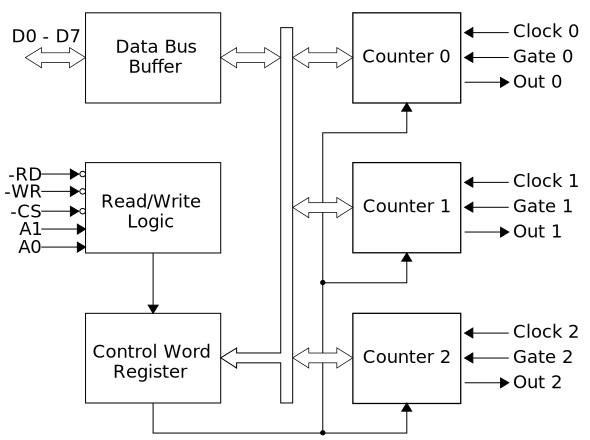
\includegraphics[scale=0.52]{img/Intel_8253_block_diagram.pdf} \end{textblock}
\end{frame}

\begin{frame}[t]
    \frametitle{Keyboard controller}
    El integrado \texttt{8042} o controlador PS/2 permite controlar tanto el teclado como el mouse.
    \pause
    \begin{block}{Uso}
    \begin{itemize}
        \item[-] Leemos teclas a través del puerto \textbf{0x60} (\textbf{in al, 0x60})
        \item[-] Obtenemos un \textbf{scan code}
    \end{itemize}
    \pause
    \end{block}
    \begin{block}{\textbf{Scan code}: Único para cada tecla}
        El teclado genera dos interrupciones:\\
        \hspace{1cm} Scancode=\texttt{0xxxxxxx} - \textbf{make}: Cuando se está presionando una tecla\\
        \hspace{1cm} Scancode=\texttt{1xxxxxxx} - \textbf{break}: Cuando se la está soltando una tecla
    \end{block}
    \pause
    \textcolor{verdeuca}{Ejemplo:}\\
    \hspace{2cm} Presionar \textbf{a} $\rightarrow$ scancode \textbf{0x1E}\\
    \pause
    \hspace{2cm} Presionar \textbf{b} $\rightarrow$ scancode \textbf{0x30}\\
    \pause
    \hspace{2cm} Soltar \textbf{a} $\rightarrow$ scancode \textbf{0x9E} (\texttt{0x1E + 0x80})
\end{frame}

\begin{frame}[fragile]
\frametitle{Rutinas del PIC}
    El archivo \texttt{pic.h} contiene las rutinas para controlar el PIC.\\
    \begin{itemize}
    \small
        \item \textbf{pic\_reset}: Remapea los PICs a indices despues de las excepciones del procesador.
        \pause
        \item \textbf{pic\_enable}: Habilita los PICs para que generen interrupciones.
        \item \textbf{pic\_disable}: Deshabilita los PICs para impedir que generen interrupciones.
        \pause
        \item \textbf{pic\_finish1}: Indica al PIC1 que fue atendida una interrupción.
        \item \textbf{pic\_finish2}: Indica al PIC2 que fue atendida una interrupción.
    \end{itemize}
    \pause
    \begin{block}{\small Código para activar interrupciones externas}
    \vspace{-0.3cm}
    \small
    \begin{verbatim}
    call pic_reset  ; remapear PIC
    call pic_enable ; habilitar PIC
    sti             ; habilitar interrupciones
    \end{verbatim}
    \vspace{-0.7cm}
    \end{block}
    Una vez activado el PIC debemos indicarle al procesador que debe responder interrupciones externas.
    La instrucción \textbf{sti} setea el flag de interrupciones.
\end{frame}

\begin{frame}[fragile]
\frametitle{Rutinas de interrupciones}
    Una vez activadas, nos comenzarán a llegar interrupciones del reloj (\textbf{32}) y del teclado (\textbf{33}).
    \pause
    \begin{block}{\small Código para anteder una interrupción externa}
    \vspace{-0.3cm}
    \small
    \begin{verbatim}
    _isr:
        pushad
        ...
        call pic_finish1
        ...
        popad
        reti
    \end{verbatim}
    \vspace{-0.7cm}
    \end{block}
    Cuando atendemos una interrupción generada por el PIC. \\ Debemos notificarle que ya la atendimos. Para eso usamos rutina \textbf{pic\_finish1}
\end{frame}

\begin{frame}[fragile]
\frametitle{Rutinas de interrupciones de ejemplo}
    \begin{block}{\small Código ejemplo para anteder el reloj}
    \vspace{-0.3cm}
    \small
    \begin{verbatim}
    _isr32:
        pushad
        call pic_finish1 ; Indica que la interrupcion fue antendida
        call nextClock   ; Imprimir el reloj del sistema
        popad
        iret
    \end{verbatim}
    \vspace{-0.7cm}
    \end{block}
    \vspace{-0.1cm}
    \begin{block}{\small Código ejemplo para anteder el teclado}
    \vspace{-0.3cm}
    \small
    \begin{verbatim}
    _isr33:
        pushad
        in al, 0x60        ; Captura una tecla
        push eax
        call printScanCode ; Rutina para imprimir el ScanCode
        add esp, 4
        call pic_finish1   ; Indica que la interrupcion fue antendida
        popad
        iret
    \end{verbatim}
    \vspace{-0.7cm}
    \end{block}
\end{frame}

\begin{frame}[fragile]
    \frametitle{Bibliografía: Fuentes y material adicional}
    \begin{itemize}
    \item Convenciones de llamados a función en x86: \\
    \url{https://en.wikipedia.org/wiki/X86_calling_conventions}
    \item Notas sobre System V ABI: \\
    \url{https://wiki.osdev.org/System_V_ABI}
    \item Documentación de NASM: \\
    \url{https://nasm.us/doc/}
    \item Artículo sobre el flag \texttt{-pie}: \\
    \url{https://eklitzke.org/position-independent-executables}
    \item Documentación de System V ABI: \\
    \url{https://uclibc.org/docs/psABI-x86_64.pdf}
    \item Manuales de Intel: \\
    \url{https://software.intel.com/en-us/articles/intel-sdm}
    \end{itemize}
\end{frame}

\begin{frame}[plain]
    \begin{center}
    \vspace{2cm}
    \huge ¡Gracias!\\
    \vspace{2cm}
    \normalsize Recuerden leer los comentarios al final de \\ este video por aclaraciones o fe de erratas.
    \end{center}
\end{frame}

\end{document}

%\tiny
%\begin{table}
%	\centering
%		\begin{tabular}{|c|c|l|l|l|l|}
%		\hline5
%		Vec. & Mne & Description & Type & Error  & Source \\ 
%		No.  &     &             &      & Code & \\
%		\hline
%		0 & \#DE & Divide Error & Fault & No & DIV and IDIV instructions. \\
%		1 & \#DB & RESERVED & Fault/ Trap & No & For Intel use only. \\
%		2 & - & NMI Interrupt & Interrupt & No & Nonmaskable external \\
%		  &   &               &           &    & interrupt. \\
%		3 & \#BP & Breakpoint & Trap & No & INT 3 instruction. \\
%		4 & \#OF & Overflow & Trap & No & INTO instruction. \\
%		5 & \#BR & BOUND Range Exceeded & Fault & No & BOUND instruction. \\
%		6 & \#UD & Invalid Opcode & Fault & No & UD2 instruction or \\
%			&   &               &           &    & reserved opcode.1 \\
%		7 & \#NM & Device Not Available & Fault & No & Floating-point \\
%		&   &               &           &    & or WAIT/FWAIT instruction. \\
%		 	&      & (No Math Coprocessor) &  &  &  \\
%		8 & \#DF & Double Fault & Abort & Yes & Any instruction \\
%		&   &               &           & (zero)   &  that can generate an exception, \\
%		&   &               &           &    &  an NMI, or an INTR. \\
%		9 & - & Coprocessor Segment Overrun & Fault & No & Floating-point instruction.2 \\
%		10 & \#TS & Invalid TSS & Fault & Yes & Task switch or TSS access. \\
%		11 & \#NP & Segment Not Present & Fault & Yes & Loading segment registers \\
%		&   &               &           &    & or accessing system segments. \\
%		12 & \#SS & Stack-Segment Fault & Fault & Yes & Stack operations and SS \\
%		&   &               &           &    & register loads. \\
%		13 & \#GP & General Protection & Fault & Yes & Any memory reference and \\
%		&   &               &           &    & other protection checks. \\
%		14 & \#PF & Page Fault & Fault & Yes & Any memory reference. \\
%		15 &  & (Intel reserved. Do not use.) & & No & \\
%		16 & \#MF & x87 FPU Floating-Point Error & Fault & No & x87 FPU floating-point or \\
%		&   &               &           &    &  WAIT/FWAIT instruction. \\
%		17 & \#AC & Alignment Check & Fault & Yes (Zero) & Any data reference in memory.3 \\
%		18 & \#MC & Machine Check & Abort & No & Error codes (if any) and source \\
%		&   &               &           &    &  are model dependent.4 \\
%		19 & \#XM & SIMD Floating-Point Exception & Fault & No & SSE/SSE2/SSE3 \\
%		&   &               &           &    & floating-point instructions5 \\
%		20-31 & - &         &           &    & Intel reserved. Do not use. \\
%		\hline
%		32-255 & - & User Defined (Non-reserved) & Interrupt &  & External interrupt or \\
%		&   &               &           &    & INT n instruction. \\
%		\end{tabular}
%\end{table}
